\chapter[Synergy with WFIRST]{Synergy with WFIRST}
\def\chpname{wfirst}\label{chp:\chpname}

Chapter editor:
\credit{jasondrhodes}.

Contributing authors:
\credit{rubind},
\credit{davidpbennett},
\credit{mtpenny},
{\it Rachel Street}.

\section*{Summary}
\addcontentsline{toc}{section}{~~~~~~~~~Summary}

WFIRST will launch in $\sim$ 2025 for a 5 year mission to explore dark energy, find and characterize exoplanets, and take wide, deep infrared surveys of the galactic and extragalactic sky.  WFIRST was recognized by the Astro2010 Decadal Survey as an excellent NIR complement to LSST's optical capabilities. More recent work has recognized the strong synergy these two projects will have in helping to address cosmological questions in the 2020s \citep{2015arXiv150107897J}.
  Together, the two observatories can accomplish significantly more (and better) science than either can alone in the areas of weak lensing, large-scale structure studies, strong lensing, supernova studies, exoplanet investigations,  and photometric redshift determination. Accomplishing this will require coordinated observations.  We have identified three areas of proposed coordination: 1. Early coverage of the $>2000$ square degree WFIRST High Latitude Survey to the full optical depth for enhanced photometric redshifts for both LSST and WFIRST; 2. Coordinated LSST optical observations in the WFIRST supernova discovery fields; 3. Precursor, simultaneous, and follow-up observations of the WFIRST microlensing fields near the galactic bulge.

  We note here that the focus of the WFIRST  input to this paper is on suggesting changes or enhancements to the LSST observing strategy (cadence or survey overlap) that will provide mutual benefit for WFIRST and LSST.  The observing strategy suggestions here are not exhaustive of the possibilities for synergy between WFIRST and LSST; rather the suggestions here are based on the planned primary WFIRST surveys that are driving the WFIRST mission requirements.  As the plans and possibilities for WFIRST Guest Observer surveys evolve, and the ideas for additional science investigations that will make use of planned WFIRST survey data mature, the community should continue to look for areas of survey synergy.  Both WFIRST and LSST should consider survey modifications that would increase the global combined science output of the two surveys.


% --------------------------------------------------------------------

\section{Introduction}
\label{sec:wfirst:intro}

% Introduce, with a very broad brush, this chapter's science projects,
% and why it makes sense for them to be considered together.

The Wide Field Infrared Survey Telescope (WFIRST) is a NASA mission that
entered Phase A in February 2016.  WFIRST was the highest recommendation
for large space missions in the 2010 New Worlds New Horizons Decadal
Survey.  That recommendation envisioned a wide-field observatory with
near infrared (NIR) capabilities to complement LSST's optical
capabilities; the Decadal Survey recognized the obvious synergy between
WFIRST and LSST.  WFIRST's design has evolved since 2010 and the design
being pursued for a mid-2020s launch uses an existing $2.4$m telescope
donated to NASA, giving WFIRST capabilities not envisioned by the
Decadal Survey.  WFIRST has 3 primary science objectives:

\begin{itemize}
\item Determine the nature of the dark energy that is driving the
current accelerating expansion of the universe using a combination of
weak lensing, galaxy clustering (including Baryon Acoustic Oscillations
and Redshift Space Distortions), and supernovae type Ia (SN).
\item Study exoplanets through a statistical microlensing survey and via
direct imaging and spectroscopy with a coronagraph.
\item Perform NIR surveys of the galactic and extragalactic sky via a
Guest Observer program.
\end{itemize}

WFIRST will be at L2 to enable the thermal stability needed for the
precise astrometric, photometric, and morphological measurements
required for these science goals. The baseline WFIRST mission
architecture is described in detail in the final report of the WFIRST
Science Definition Team \citep{2015arXiv150303757S}
%(arxiv/1503.03757).
The WFIRST Wide Field
Instrument(WFI) has a NIR focal plane with a $\sim0.28$ square degree
field of view made up 18 4k$\times$4k Teledyne H4RG NIR detectors and will
have imaging capabilities from $0.5-2$ microns and grism spectroscopy
capabilities from $1-2$ microns with $R\sim461\lambda$.  The WFI
also contains an Integral Field Channel (IFC) spectrometer with $R\sim100$
resoluton over the range $0.6-2$ microns for SN follow up. The exoplanet
coronagraph will have imaging ($0.43-0.97$ microns) and spectroscopic
($0.6-0.97 $ microns) capabilities with a contrast ratio of 1 part in a
billion.

WFIRST's  5 year primary mission is envisioned to have $\sim2$years dedicated to a
$\sim2200$ square degree High Latitude Survey (HLS) for weak lensing and
galaxy clustering,  $\sim1$ year of microlensing observations divided into 6
seasons, $\sim0.5$ years of SN search and follow-up, $\sim0.8$ years dedicated to
the coronagraph and the remaining time dedicated to competitively selected Guest
Observer observations. WFIRST has no expendables that would prevent an
extended mission of 10 years or longer, and an extended mission will likely be
given over entirely to Guest Observer observations.

The synergy with LSST is very promising indeed. In this chapter we aim
to  lay out three  specific projects in the three main WFIRST science
areas, and test the simulated LSST Observing
Strategies for their performance in each case. Then, we use these
results to design a suite of modified LSST Observing Strategies, which
we propose as new \OpSim simulation runs.


\navigationbar


% --------------------------------------------------------------------

% ====================================================================
%+
% SECTION:
%    WFIRST_weaklensing.tex
%
% CHAPTER:
%    wfirst.tex
%
% ELEVATOR PITCH:
%
%
% AUTHORS:
%    Jason Rhodes @jasondrhodes
%-
% ====================================================================

\section{Cosmology with the WFIRST HLS and LSST}
\def\secname{\chpname:weaklensing}\label{sec:\secname}

\credit{jasondrhodes}

WFIRST's High Latitude Survey (HLS) will cover
2200 square degrees in 4 NIR photometric filters
(3 of which will be sufficiently sampled for weak lensing shape
measurements) and NIR grism spectroscopy.  The benefits of overlapping
spectroscopic and photometric surveys for dark energy constraints and
systematics mitigation are strong.  The primary scientific driver of the
photometric portion of the WFIRST HLS is weak gravitational lensing,
but there is a wide range of ancillary science that will be possible
with the publicly available WFIRST HLS data (see for instance, the SDT
report mentioned above).  However, the requirements on the HLS are
largely set by constraints from weak lensing measurements.  Each galaxy
in the WFIRST weak lensing survey needs to have an accurate photometric
redshift.  This requires optical photometry that reaches the depth of
the NIR photometry WFIRST will acquire ($J~27AB$).  \emph{Thus, the
WFIRST weak lensing survey will require the full  10-year LSST depth in
4 optical bands for optimal photometric redsfhift determination}.

There is strong benefit not just to WFIRST, but to LSST, in coordinating
observations of the WFIRST HLS survey field. The combination of
full-depth LSST data and WFIRST HLS NIR data will provide the gold
standard in photo-zs.  Furthermore, WFIRST grism observations over the
same area will provide many millions of high quality slitless spectra
and WFIRST's IFC can be run in parallel with WFI observations to provide
many more very accurate spectroscopic redshifts in the survey area.
Thus, the WFIRST photometric data will help to provide better LSST
photo-zs and  WFIRST will also provide many of the spectra needed as a
training set to calibrate the photo-zs for both missions.  A further
benefit to LSST might be the reduced need for LSST observations at the
reddest end of the LSST wavelength range (the $z$ and $y$ filters), where
both the atmosphere and the physics of CCDs make ground-based
observations less efficient than what WFIRST can achieve. Further work is needed to quantify this benefit, especially as the WFIRST proposed filter set is evolving.Finally, the
joint processing of LSST and WFIRST data will provide better object
deblending parameters than LSST can achieve alone; WFIRST will be able
to provide a morphological prior for the deblending of LSST images.

% --------------------------------------------------------------------

\subsection{Measuring Dark Energy Parameters}
\label{sec:\secname:targets}

The goal in this science project would be to measure Dark Energy parameters from various weak lensing
probes, capitalizing on the improved photometric redshifts that a joint
analysis of LSST and WFIRST photometry would provide. A useful
Figure of Merit is the usual Dark Energy Task Force figure of merit,
quantifying the available precision on the equation of state
parameters $w_0$ and $w_a$. For example, we are interested in
improvements in the weak lensing DE FoM as the LSST photometric redshifts
and galaxy shapes are improved over the whole LSST survey area
via joint analysis with WFIRST. We are also interested in increasing the
WFIRST DE FoM as quickly as possible.
Indeed, the basic problem we face is one of timing: being able to combine
the WFIRST data with the LSST sooner will accelerate the production of
cosmological results.

Therefore, we propose an acceleration of the LSST survey over about $10\%$ of the
LSST survey area (the $\sim2200$ WFIRST HLS) such that the full LSST ten
years survey depth is reached on a timescale that maximizes the joint
usefulness of LSST and WFIRST data on that area.  Assuming the two year
WFIRST HLS is taken in the first four years of a WFIRST mission that
launches in 2024, this would require reaching full LSST depth over that
area in $\sim2028$ rather than $\sim2032$. Since the HLS area is roughly
$1/8$ as large as the LSST ``Main Survey"'' region, this could be
achieved by devoting 1.25 years of LSST observations to the HLS area,
assuming that it covers a wide enough range of Right Ascension.  More
practically, it could be achieved by devoting 25\% of LSST observing
time to this area during each of the first 5 years of the LSST survey,
which doubles the time it would naturally be observed during those years
at a modest reduction in coverage of the rest of the Main Survey area
during that time period.   Given existing plans to speed up the LSST
cadence over small sub-areas of the LSST survey, this may only require
coordination of the locations of the accelerated LSST area and the
WFIRST HLS. As LSST and WFIRST progress, there is a mutual benefit in
continuing discussions about the optimal joint observation schedule.


A simple, first order diagnostic metric would be the amount of LSST/WFIRST
overlapping survey area that reaches the full LSST depth when the WFIRST
HLS is completed.  Such a metric is straightforward, but not
able to be meanigfully encoded until the 2020s, when the WFIRST launch date and survey
plan is more definite.  Strawman survey plans could, however, be
evaluated to help with LSST schedule planning.
A slightly more complicated metric could include
the pace at which the overlapping LSST/WFIRST survey areas are both
taken to full depth, since this would make each data set maximally
useful to the US community (or anyone with immediate access to both
WFIRST and LSST data).  WFIRST data is unlikely to have any proprietary
period.  Current plans call for the WFIRST HLS to be conducted in
multiple passes, but the exact survey pattern is still undecided, so this
metric is also not quantifiable yet.

There may be some reduced need for the the LSST reddest bands in the
WFIRST HLS overlap area, which should also be folded into the metric.
We note that
the default survey strategy would only achieve the full LSST photometric
depth over the WFIRST HLS after 10 years of survey ($\sim2032$).



% % --------------------------------------------------------------------
%
% \subsection{OpSim Analysis}
% \label{sec:\secname:analysis}
%
%
% % --------------------------------------------------------------------

\subsection{Discussion}
\label{sec:\secname:discussion}

Increasing the cadence of the LSST survey over $\sim10\%$ of the LSST
survey has science benefits that go far beyond the LSST/WFIRST synergy
described here: an observing strategy that met the joint WFIRST/LSST cosmology goals could
also provide the kind of ``rolling cadence'' favored by other science teams.
There are benefits to certain aspects of time-domain
science.  Every effort should be made to coordinate all discussions of
increased survey cadence (resulting in full LSST depth well before 10
years) over sub-areas of the LSST survey footprint.  Specific attention
should be paid to whether the accelerated portions of the LSST survey
can completely overlap the WFIRST HLS, and whether the position of the
WFIRST HLS can be determined, in part, by other science drivers within
LSST.  This will require close LSST and WFIRST coordination at the
Project levels.

% % --------------------------------------------------------------------

\subsection{Conclusions}
\label{sec:\secname:conclusions}

Even before implementing the metrics decsribed above, we can offer
tentative answers to the ten questions posed in
\autoref{sec:intro:evaluation:caseConclusions}:

\begin{description}

\item[Q1:] {\it Does the science case place any constraints on the
tradeoff between the sky coverage and coadded depth?}

\item[A1:] WFIRST requires the full 10 year LSST depth over the $\sim$ 2000 square degree WFIRST High Latitude Survey.

\item[Q2:] {\it Does the science case place any constraints on the
tradeoff between uniformity of sampling and frequency of  sampling? For
example, a rolling cadence can provide enhanced sample rates over a part
of the survey or the entire survey for a designated time at the cost of
reduced sample rate the rest of the time (while maintaining the nominal
total visit counts).}

\item[A2:] The WFIRST HLS synergy does not place constraints on the uniformity of time sampling.

\item[Q3:] {\it Does the science case place any constraints on the
tradeoff between the single-visit depth and the number of visits?}

\item[A3:] The WFIRST HLS only places requirements on the total depth in
the 5 LSST photometric filters.

\item[Q4:] {\it Does the science case place any constraints on the
Galactic plane coverage (spatial coverage, temporal sampling, visits per
band)?}

\item[A4:] No: the WFIRST HLS will not be in the Galactic plane.

\item[Q5:] {\it Does the science case place any constraints on the
fraction of observing time allocated to each band?}

\item[A5:] There are multiple solutions to the allocation of depth to each of the 5 LSST and 3 WFIRST bands that will be used for optimzed photometric redshifts. This is a area of ongoing study.

\item[Q6:] {\it Does the science case place any constraints on the
cadence for deep drilling fields?}

\item[A6:] No.

\item[Q7:] {\it Assuming two visits per night, would the science case
benefit if they are obtained in the same band or not?}

\item[A7:] The WFIRST HLS is largely agnostic about the timing of the different filters.

\item[Q8:] {\it Will the case science benefit from a special cadence
prescription during commissioning or early in the survey, such as:
acquiring a full 10-year count of visits for a small area (either in all
the bands or in a  selected set); a greatly enhanced cadence for a small
area?}

\item[A8:] The WFIRST HLS synergy would be globally maximized (for both
LSST and WFIRST) if the full LSST depth in all 5 bands is reached in the
first 5 years of LSST operations.

\item[Q9:] {\it Does the science case place any constraints on the
sampling of observing conditions (e.g., seeing, dark sky, airmass),
possibly as a function of band, etc.?}

\item[A9:] The benefit to LSST of having high precision space based
galaxy shape measurements would be maximized if the observing conditions
allowed for the best possible LSST shapes for cross-calibration of shear
measurements.

\item[Q10:] {\it Does the case have science drivers that would require
real-time exposure time optimization to obtain nearly constant
single-visit limiting depth?}

\item[A10:] No.

\end{description}

% ====================================================================

\navigationbar


% ====================================================================
%+
% SECTION:
%    WFIRST_supernovae.tex
%
% CHAPTER:
%    wfirst.tex
%
% ELEVATOR PITCH:
%-
% ====================================================================

\section{Supernova Cosmology with WFIRST and LSST}
\def\secname{\chpname:supernovae}\label{sec:\secname}

\credit{rubind}

% This individual section will need to describe the particular
% discoveries and measurements that are being targeted in this section's
% science case. It will be helpful to think of a ``science case" as a
% ``science project" that the authors {\it actually plan to do}. Then,
% the sections can follow the tried and tested format of an observing
% proposal: a brief description of the investigation, with references,
% followed by a technical feasibility piece. This latter part will need
% to be quantified using the MAF framework, via a set of metrics that
% need to be computed for any given observing strategy to quantify its
% impact on the described science case. Ideally, these metrics would be
% combined in a well-motivated figure of merit. The section can conclude
% with a discussion of any risks that have been identified, and how
% these could be mitigated.
%
% A short preamble goes here. What's the context for this science
% project? Where does it fit in the big picture?

The WFIRST SN survey seeks to measure thousands of SNe Ia with excellent systematics control over a two-year period. The Science Definition Team (SDT) outlined a three-tiered cadenced imaging survey: wide to $z=0.4$ (27.44 square degrees), medium to $z=0.8$ (8.96 square degrees), deep to $z=1.7$ (5.04 square degrees). SNe discovered in the imaging would be followed with IFU spectrophotometry, helping to monitor changes in SN physical parameters and the extinction distribution with redshift.
% However, due to the slew time and high read noise in short exposures, the wide survey would be very inefficient, spending a bit more than half of its time on slews, while the medium survey would spend a significant fraction of its time slewing.
However, the LSST DDFs offer a path to high signal-to-noise, well calibrated, multi-band optical imaging over an even larger area than WFIRST can survey. If the wide and medium tiers are replaced with LSST DDF discoveries, then WFIRST can offer spectrophotometry (with good host-galaxy subtraction) for $\sim$ 2,000 LSST SNe, with screening spectra for $\sim$ 1-2,000 more. As the WFI and IFU operate in parallel, this survey could provide sparsely sampled NIR imaging for $\sim$ 5,000 SNe up to $z = 1$ at the same time as the spectroscopy. The joint survey would thus provide systematics control (almost certainly better than either survey alone), as well as a cross-check of LSST photometric typing and host-galaxy-only redshift assignment.


% --------------------------------------------------------------------

\subsection{Target measurements and discoveries}
\label{sec:\secname:targets}

% Describe the discoveries and measurements you want to make.
%
% Now, describe their response to the observing strategy. Qualitatively,
% how will the science project be affected by the observing schedule and
% conditions? In broad terms, how would we expect the observing strategy
% to be optimized for this science?


The targets of the measurements are related to those enumerated in
\autoref{sec:supernovae:targets}. The SNe must be detected $\sim$ 10
observer-frame days before maximum light, so that there is time for a
shallow screening spectrum before deeper spectrophotmetry around
maximum. There should be enough visits per filter so that some
photometric screening can be done before WFIRST triggers any
spectroscopy. There should be an identification of the host galaxy (if
seen), so that joint WFIRST/LSST photometric redshifts can be used to
provide a distance-limited sample (minimizing selection effects).
Finally, the light curve should continue after the SN has been sent to
WFIRST, so that important light-curve parameters (date of maximum, rise
time and decline time, etc.) can be measured.

%All these goals can be likely be met with $\sim 3$ day rest-frame cadence ($\sim 5$ observer-frame days). LSST would measure NUV to rest-frame $V$-band (with WFIRST providing redder wavelength coverage), or observer-frame $grizY$. For a plausible SN Ia (based on the rising light curve), a series of typing/sub-typing spectra would be triggered, with increasing depth, as the confidence grew that the transient was a SN Ia. DR: in my simulations, I've assumed a depth for each filter of 26th magnitude (probably not realistic for $Y$-band, but very feasible for the other filters); is this too shallow? LSST would contribute 4 transients per day to the pool of objects observed by WFIRST. In practice, the LSST DDFs will contain more SNe Ia than this, so a random sample (perhaps sculpted in redshift) should be sent for observations.


% --------------------------------------------------------------------

\subsection{Metrics}
\label{sec:\secname:metrics}

% Quantifying the response via MAF metrics: definition of the metrics,
% and any derived overall figure of merit.

The primary metrics are based on constraining cosmological parameters;
the DETF FoM is standard. For the joint observations proposed here, this
FoM increases about 20\%, from $\sim 300$ for WFIRST alone (with a Stage
IV CMB constraint) to $\sim 370$. However, the number of SNe at $z \sim
0.5$ increases by $\sim$ 50\% over a WFIRST-only survey, improving some
$w(z)$-derived FoM values by 40\%.

The cosmological metric will essentially depend on the number of SNe
meeting the above targets. It will degrade if core-collapse SNe are
mistakenly sent to WFIRST for followup, if SNe Ia are sent to WFIRST but
the LSST light curve is lost due to weather gaps, or if the cadence and
depth simply do not allow the measurement of light curve parameters.
These metrics will be strongly related to those in
\autoref{sec:supernovae:metrics}, but with more emphasis on the rising
portion of the light curve.

% --------------------------------------------------------------------

%\subsection{OpSim Analysis}
%\label{sec:\secname:analysis}

% OpSim analysis: how good would the default observing strategy be, at
% the time of writing for this science project?


% --------------------------------------------------------------------

%\subsection{Discussion}
%\label{sec:\secname:discussion}

% Discussion: what risks have been identified? What suggestions could be
% made to improve this science project's figure of merit, and mitigate
% the identified risks?

% ====================================================================
%
\subsection{Conclusions}

Here we answer the ten questions posed in
\autoref{sec:intro:evaluation:caseConclusions}. As WFIRST will only cadence a few 10's of square degrees, we assume that the overlap region will be contained in the DDFs, not in the main survey. We thus place no constraints on the main survey.

\begin{description}

\item[Q1:] {\it Does the science case place any constraints on the
tradeoff between the sky coverage and coadded depth?}

\item[A1:] In terms of direct overlap with WFIRST, there is no constraint. There are secondary considerations (such as constraining  Milky Way extinction and probing isotropy) that may prefer a larger number of square degrees, but this has not been investigated.

\item[Q2:] {\it Does the science case place any constraints on the
tradeoff between uniformity of sampling and frequency of sampling?}

\item[A2:] No constraints.

\item[Q3:] {\it Does the science case place any constraints on the
tradeoff between the single-visit depth and the number of visits
(especially in the $u$-band where longer exposures would minimize the
impact of the readout noise)?}

\item[A3:] In the DDFs, the SN Ia science would not be harmed by having longer exposures and less-frequent visits, at least if there was one observation every few days in each filter. No constraint on the main survey.

\item[Q4:] {\it Does the science case place any constraints on the
Galactic plane coverage (spatial coverage, temporal sampling, visits per
band)?}

\item[A4:] No constraints.

\item[Q5:] {\it Does the science case place any constraints on the
fraction of observing time allocated to each band?}

\item[A5:] This has not been quantitatively investigated. Based on experience with other programs, the reddest filters (z and Y) should receive the most time.

\item[Q6:] {\it Does the science case place any constraints on the
cadence for deep drilling fields?}

\item[A6:] To obtain good light curves, we would want at least one observation every few days per filter. This is also a requirement for photometric typing to obtain reasonable purity if WFIRST spectroscopy is to be triggered. Note: of all the questions, this one is the most important to the program.

\item[Q7:] {\it Assuming two visits per night, would the science case
benefit if they are obtained in the same band or not?}

\item[A7:] No benefit.

\item[Q8:] {\it Will the case science benefit from a special cadence
prescription during commissioning or early in the survey, such as:
acquiring a full 10-year count of visits for a small area (either in all
the bands or in a  selected set); a greatly enhanced cadence for a small
area?}

\item[A8:] For the DDFs, such observations might help provide deep SN-free (template) images or host-galaxy photometric redshifts. This has not been quantitatively investigated. No constraints on the main survey.

\item[Q9:] {\it Does the science case place any constraints on the
sampling of observing conditions (e.g., seeing, dark sky, airmass),
possibly as a function of band, etc.?}

\item[A9:] As long as the DDF observations reach the targeted depths, there is no benefit to the SN Ia science from having specific observing conditions.

\item[Q10:] {\it Does the case have science drivers that would require
real-time exposure time optimization to obtain nearly constant
single-visit limiting depth?}

\item[A10:] We do not currently know of any benefit to the SN Ia science from doing this.

\end{description}

% ====================================================================

\navigationbar


% ====================================================================
%+
% SECTION:
%    WFIRST_microlensing.tex
%
% CHAPTER:
%    wfirst.tex
%
% ELEVATOR PITCH:
%
%
% AUTHORS:
%    David Bennett(@davidpbennett)
%-
% ====================================================================

\section{Exoplanetary Microlensing with WFIRST and LSST}
\def\secname{\chpname:microlensing}\label{sec:\secname}

\credit{davidpbennett},
\credit{mtpenny},
\credit{poleski},
\credit{rachelstreet}.

One of the most exciting prospects of future micolensing surveys is the
characterization of the population of ``rogue'' or free-floating planets.
While recent estimates of the rogue planet abundance (Mroz et al. 2017 in prep)
 have cast doubt on the large population of rogue planets inferred by
\citet{2011Natur.473..349S}, they have clearly demonstrated that microlensing surveys
have the sensitivity necessary to detect them. Firm detections of the rogue
planet population that might be predicted by planet formation simulations
awaits the accumulation of sufficient survey duration for giant rogue planets,
and the WFIRST microlensing survey for smaller planets~\citep{2015arXiv150303757S,2017arXiv170408749B}.
% of discovery to come out of gravitational
%microlensing surveys is the discovery of a large population of ``rogue''
%planets by the MOA Collaboration \citep{2011Natur.473..349S}, though more
%recent analysis by the OGLE Collaboration (Mroz et al. 2017 in prep) does not confirm this result. Nevertheless, WFIRST will detect many rogue planets between Mars and Jupiter mass even if their abundance is more than an order of magnitude smaller than inferred by MOA or a factor of a few smaller than expected from theoretical studies~\citep{2015arXiv150303757S, 2017arXiv170408749B}.

Microlensing's rogue planets
are isolated in the sense that no host star can be detected
by microlensing. Depending on the peak magnification and light curve
coverage, this can imply that a host must be $> 10\,$AU or $> 100\,$AU away,
and \citet{2012ApJ...757..119B} have argued that the median separation
of possible host stars is likely to be $> 30\,$AU. The presence and properties
of a host star can be constrained either with WFIRST's diffraction limited survey images separated by the mission duration, or adaptive optics observations on large telescopes ($\ge 8$~m) taken $4$--$8$ years after the rogue planet event~\citep{2016JKAS...49..123G,2016AJ....152...96H}.
%Further observations by both the MOA and OGLE collaborations provide
%a qualitative confirmation of this result, as dozens of additional
%short timescale events have been discovered by the MOA and OGLE
%alert systems, but full details of the implied rogue planet
%populations  will only come from detailed analyses of both the MOA
%and OGLE samples.

A major weakness with the microlensing survey data sets that can be used to detect rogue planets is that, thus far, the properties
of the population can only been inferred by their Einstein radius
crossing time, $t_{\rm E}$, distribution. But, the Einstein radius crossing
time depends not only on the lens mass, but also on its distance and
transverse velocity. As a result, we cannot directly infer the mass or distance
distribution of the rogue planet sample.

Our understanding of the rogue planet distribution can be greatly improved
by measuring the microlensing parallax effect \citep{1992ApJ...392..442G,1995ApJ...454L.125A}.
Combining $t_{\rm E}$ with the microlens parallax $\pi_{\rm E}$ yields a mass-distance relationship, a narrower range of possible lens masses and a projection of the lens-source relative velocity, which can in certain cases be used to identify the lens as belonging to the Galactic disk or bulge~\citep{2015ApJ...802...76Y}. The mass and distance of the lens can be uniquely solved for if, in addition to parallax, the angular diameter of the Einstein ring can be measured via finite source effects \citep{1994ApJ...424L..21N}. Finite source effects will be measured in a substantial fraction of events involving bound and free-floating planets.
%The microlensing parallax effect can be described
%by the transverse relative lens-source velocity, ${\bf v}_{\rm \perp}$, projected
%to the position of the observer,
%\begin{equation}
%\tilde{\bf v} = {\bf v}_{\rm \perp} D_S/(D_S-D_L) \ , \label{eq-vp}
%\end{equation}
%where $D_L$ and $D_S$ are the lens and source distances, respectively.

Typically, microlensing parallax
is measured using the orbital motion of the Earth, but it can also be
measured using light curve observations from telescopes at different locations
in the Solar System \citep{2007ApJ...664..862D,2015ApJ...804...20C} or
even different locations on Earth \citep{2009ApJ...698L.147G}. In the
case of microlensing by planetary mass objects, the event durations are
too short to allow a significant light curve change due to the Earth's
orbital motion, but near simultaneous observations from Earth and a
satellite orbiting at the Earth-Sun L2 point (where WFIRST will orbit) allows the measurement of microlensing parallax signals for planetary mass
lenses \citep{2003ApJ...591L..53G}. The principles of the technique are identical to those employed by the {\it K2} Campaign 9 microlensing parallax survey~\citep{2016PASP..128l4401H,2016AJ....152...96H,2017AJ....153..161P}.
\autoref{fig-lc} shows an example of the light curves for one of the
rogue planets with a mass determined by simultaneous WFIRST and LSST
observations.

%When a microlensing parallax signal is measured, the $\tilde{\bf v}$ value
%can generally distinguish between bulge and disk lenses, as $\tilde{\bf v}$
%generally points in the direction of the Galactic disk rotation and has
%a magnitude of $\tilde{v} \ltsim 200\,$km/sec for a lens in the
%disk, while for a lens in the bulge, the magnitude of the projected velocity
%is $\tilde{v} \gtsim 200\,$km/sec. A microlensing parallax measurement also
%yields a mass distance relationship,
%\begin{equation}
%   M_{\rm L} = {\tilde{v}^2 t_{\rm E}^2 c^2 \over 4 G} {D_S-D_L \over D_L D_S} \ .
%   \label{eq-m_vt}
%\end{equation}
%Because the $\tilde{\bf v}$ value places a fairly strong constraint
%on $D_L$ and the source is very likely to be in the bulge, equation~\ref{eq-m_vt}
%generally provides a good constraint on the lens mass. But, for some
%events, we can do even better. For high magnification events or events
%with low-mass lenses, the finite angular size of the source star is
%resolved, and the light curve provides a measurement of the source
%radius crossing time, $t_*$. This allows the angular Einstein radius
%to be determined, $\theta_{\rm E} = t_{\rm E} \theta_*/t_*$, where the angular
%source radius, $\theta_*$ can be determined from the color and brightness
%of the source star \citep{2014AJ....147...47B}. When both $\tilde{v}$ and
%$\theta_{\rm E}$ are known, the mass of the lens is measured to be
%\begin{equation}
%M_{\rm L} = {c^2\over 4G} \tilde{v} t_{\rm E} \theta_{\rm E} = {\theta_{\rm E}\tilde{v} t_{\rm E} \over (8.14\,{\rm mas\, AU})} M_{\odot} \ .
%\label{eq-m}
%\end{equation}
%Figure~\ref{fig-lc} shows an example of the light curves for one of the
%rogue planets with a mass determined by simultaneous WFIRST and LSST
%observations.

\begin{figure}[t]
\centering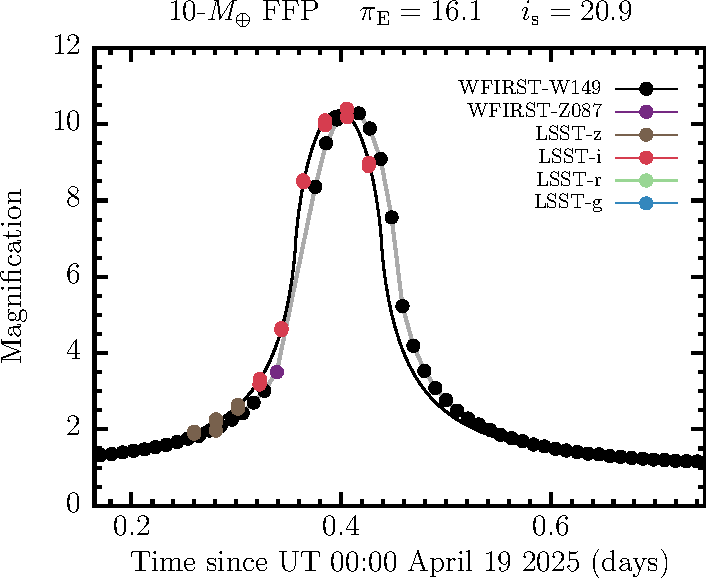
\includegraphics[width=0.5\linewidth]{figs/WFIRST/lsst_lsstm+10_0_7220351_320_det_lc.pdf}
\caption{A simulated light curve of a $10 M_{\oplus}$ planet with a microlensing parallax
mass measurement from simultaneous WFIRST and LSST observations. The short duration of WFIRST planetary microlensing events and the high extinction in WFIRST's fields requires high-cadence (ideally every $15$-$30$ min) observations in the redder bands ($i$ or $z$, preferably). During WFIRST observations around the equinoxes, the LSST-WFIRST microlensing field will only be visible for a few hours per night.}
\label{fig-lc}
\end{figure}

WFIRST planetary microlensing events will greatly improve our
understanding of not only rogue planets population but also of planets in wide orbits similar to those of
Uranus or Neptune and with a wide range of masses~\citep{2015arXiv150303757S}. Such cold planets
cannot be studied using techniques other than microlensing~\citep[e.g.,][]{2012ARAA..50..411G} and
WFIRST gives us a unique opportunity to detect a statistically significant
number of wide orbit planets.
%Even though the wide orbit planets will be detected,
%their properties may not be well constrained by WFIRST or it may be hard to distinguish
%between a wide orbit planet and a rogue planet, particularly for planets on the widest
%orbits or when the source trajectory does not closely approach the host star.
%The two main parameters that can be derived for bound planets are
%the mass ratio, $q$, and the projected separation, $s$, in units of Einstein radius.
A wide-orbit planet adds an additional peak to the otherwise
standard microlensing light curve produced by the host star that occurs a few Einstein crossing timescales before or after the host event's peak~\citep[e.g.,][]{2014ApJ...795...42P}. Typical host event timescales are ${\sim}25$~days, so it will be common for the host peak of a wide-orbit planet discovered by WFIRST to lie outside of WFIRST's $72$~day observing window, but inside the time when LSST can observe it. Without ground-based observations outside the WFIRST window, the properties of many wide-orbit planet detections by WFIRST will be poorly constrained, particularly the mass ratio of the planet to its host, and its projected separation from the host. However, deep, low-cadence LSST
monitoring of the WFIRST microlensing field over whole bulge observing season
will reveal the peaks of planet host microlensing events that are unobservable
to the WFIRST and will enable measurement of the projected separation and mass ratio.
%help to constrain projected separation and mass ratio.

%The time separation of the two peaks, $\Delta t$, is directly related
%to the planet projected separation:
%\begin{equation}
% \Delta t =  t_{\rm E}(s - {1/s}) \ .
%\end{equation}
%sTypical value of $t_{\rm E}$ is $25~{\rm days}$, hence, for a wide
%separation planet ($s$ on the order of a few) $\Delta t$ will be
%comparable to the length of a single WFIRST session i.e., $72~{\rm days}$.
%Even though WFIRST will be able to observe the planetary anomaly,
%it may not observe the host event and hence poorly constrain planet properties.


% --------------------------------------------------------------------

\subsection{A Proposed Observing Strategy}
\label{sec:\secname:proposal}

Based on the desiderata above, we
propose simultaneous high cadence observations of the WFIRST microlensing fields
by LSST during each
of the six 72-day WFIRST exoplanet microlensing survey sessions. These
will allow microlensing parallax measurements to determine the distances
and masses of a representative sub-sample of the rogue planets found by
the WFIRST microlensing survey. These measurements will be crucial for
the interpretation of WFIRST's rogue planet discoveries, and they
cannot be obtained by another method.

We also propose continuous monitoring of the WFIRST microlensing fields
at a cadence of one observation per day
starting a year before and ending a year after the WFIRST microlensing survey.
This will allow us to constrain the presence of a host star for rogue planet candidates and,
if the host is detected, measure the planet-host mass ratio and projected separation.

A single LSST pointing, centered on the WFIRST microlensing
fields, would cover all 10 WFIRST microlensing fields.

For our preliminary estimates of the high-cadence observing, we assume
that the bulge is observed every 30 minutes when the bulge is at
an airmass of $< 2.5$ for 76-day observing runs (each 72-day WFIRST observing
season plus 2 days on either side). Each visit consists of 3 exposures,
one 2 sec exposure followed by two 15 sec exposures. With a 2 sec readout
and 1 sec for the shutter to open and close, this comes to 39 sec on target
per visit (since the final readout can be done while slewing).
If we assume a 30 deg slew in Azimuth before and after each microlensing pointing, the slews
to and from the target should take 22 sec, which is 12 sec above the average. So,
each visit will take 61 sec out of the regular observing sequence.
The number of observations per night, assuming a 30 minute cadence, for
a Spring 2025 observing session are given in \autoref{tab:wfirst_ml_survey}. We will require
that these observations be taken in the $riz$ or $y$ filters with at
least 3 (or 0) observations in each filter per night. The total number
of observations with this observing plan is 649 or 11.0 hour per
76-day observing session or 3894 observations and 66.0 hours for
all the high cadence observations that we propose.

\begin{table}
\begin{tabular}{ c c }
  {\bf Dates} & {\bf Number of observations per night}\\
\hline
Feb 10-16     &  3 \\
Feb 17-23     &  4 \\
Feb 24-Mar 1  &  5 \\
Mar 2-8       &  6 \\
Mar 9-14      &  7 \\
Mar 15-21     &  8 \\
Mar 22-28     &  9 \\
Mar 29-Apr 4  & 10 \\
Apr 5-10      & 11 \\
Apr 11-17     & 12 \\
Apr 18-24     & 13 \\
Apr 25-28     & 14 \\
\end{tabular}
\caption{Observations per night at 30 minute cadence for a Spring
WFIRST microlensing survey. This is also approximately the number of minutes required per night for exoposure time and overheads.}
\label{tab:wfirst_ml_survey}
\end{table}

These observing plans can be altered by changing the cadence of the high
cadence observations from once every 30 minutes to once every 15, 60,
or 120 minutes, or we could change the number of WFIRST microlensing
observing seasons that were covered. We have not yet simulated the
different observing cadences, however.

The low-cadence (1 observation per day) observations taken when WFIRST
is not observing, would consist of 1270 visits if we assume that
the observations are not taken during the time when the $u$ filter is
on the telescope (this is assumed to be 1/6 of the time). The low-cadence
off-season observations then total 21.5 hours. Low- and high-cadence
observations will take a total of 87.5 hours over 8 years.



% --------------------------------------------------------------------

\subsection{Metrics}
\label{sec:\secname:metrics}

\subsubsection{High-cadence observations}

\autoref{tab:wfirst_ml_results}
shows the results of our simulations of the combined proposed WFIRST-LSST
observing program. We assume that there is 1 planet per main sequence
star at each of $1\,M_\oplus$, $10\,M_\oplus$, and $100\,M_\oplus$.
%This is the 1-$\sigma$ lower limit found by \citet{2011Natur.473..349S} at
%$M_{\rm L} \approx 300\,M_\oplus$, and the rogue planet mass function is
%thought to increase toward lower masses, so this is a conservative
%assumption.
The first row gives the number of events that will be
observed by WFIRST. The second row gives the number of these events
with source SDSS-$i \leq 23$, which were the only events included in the
LSST simulations. The third and fourth rows give the number of these events
with LSST-WFIRST microlensing parallax measurements and the number
with full mass measurements. It is this row that indicates the
value of the LSST observations.

\begin{table}
\begin{tabular}{lcccc}
Category & $100\,M_\oplus$ & $10\,M_\oplus$ & $1\,M_\oplus$ & Total \\
\hline
WFIRST-events    &   417   &         127    &         33    &  577  \\
$i \leq 23$      &    88   &          30    &         13    &  131  \\
$\pi_{\rm E}$ measured &    22   &           8.2  &          2.7  &   32.9 \\
$M_{\rm L}$ measured   &    5.9  &           3.4  &          1.5  &   10.8 \\
\end{tabular}
\caption{Number of rogue planets of the given mass detected, assuming
one such planet per main sequence star, and our proposed LSST observation
program.}
\label{tab:wfirst_ml_results}
\end{table}

One can see from the final column that the LSST observations should
yield more than 30 rogue planet microlensing parallax measurements and
more than 10 rogue planet mass measurements.
%
These are measurements that cannot be made by other methods, as there is
currently no other known way to measure the mass distribution and abundance
of dark, isolated objects.
% \textbf{THE PREVIOUS SENTENCE NEEDS MORE JUSTIFICATION.}
%
In addition, this program would
also yield masses for a somewhat larger number of bound planets
\citep{2003ApJ...591L..53G}, although many of these will have their
masses determined by other means as well.

For a proxy for a Figure of Merit, we select the product of the numbers of
rogue planet microlensing parallax measurements $\pi_{\rm E}$
and rogue planet mass measurements $M_{\rm L}$.
% Added by PJM:
We expect this quantity to be simply related to the ultimate precision
on any rogue planet population hyperparameter we may try to infer from
the LSST-WFIRST sample.
Some additional
work is still needed to test and develop this metric so that it can be easily incorporated into the \MAF based on \OpSim runs.
The value of this product is 355 for our straw man program.


\subsubsection{Low-cadence observations}

LSST observations will improve models for WFIRST planetary events
in a number of ways but here we focus on detection of the planet
host peak if it was missed and poorly constrained by WFIRST. We simulate
a population of planets with masses of $0.1\,M_\oplus$, $1\,M_\oplus$,
and $10\,M_\oplus$ that follow logarithmic mass function with
normalization extrapolated from \citep{2012Natur.481..167C}. We narrow the sample of
planets detected by WFIRST in a number of steps. First, we reject the events
with host peak during the LSST high-cadence observations, i.e., during one of six
76-day long campaigns. Second, we exclude the events for which flux increase
during the WFIRST observing season is at least $0.75$ of the event maximum
flux increase, because in these cases WFIRST
data will strongly constrain the host peak even though it is not fully observed.
Third, we require at least a single LSST observation within $\pm0.05t_{\rm E}$ of
the host peak and the magnified source flux to be brighter than SDSS-$z$ of $23~{\rm mag}$.
The expected number of $0.1\,M_\oplus$, $1\,M_\oplus$, and $10\,M_\oplus$
planets for which host peak is detected are 2.1, 8.7, and 36.9, respectively.
We chose a sum of those as a proxy for a Figure of Merit. For the observing strategy
presented above the value of this Figure of Merit is 47.7. If a maximum airmass is chosen to be
2.0 instead of 2.5, then the requested time decreases by $6\%$ and Figure of Merit decreases by $12\%$.
The metric is based solely on the distribution of peak times and source magnitudes
for a given WFIRST simulation, so once this is set, the metric can
be easily computed for any \OpSim run.


% Quantifying the response via MAF metrics: definition of the metrics,
% and any derived overall figure of merit.

% % --------------------------------------------------------------------
%
% \subsection{OpSim Analysis}
% \label{sec:\secname:analysis}
%
% OpSim analysis: how good would the default observing strategy be, at
% the time of writing for this science project?
%
%
% % -------------------------------------------------------------------- % %

\subsection{Discussion}
\label{sec:\secname:discussion}

The rough estimates of our metrics and Figure of Merit given above were
carried out using a very simple model for the LSST observations we
have proposed. We would hope to refine this analysis using the output
of an \OpSim run where the WFIRST+LSST microlensing program was included
as an additional special survey, and our Figure of Merit coded in the
MAF. We do not expect the impact of this special survey on other science cases
to be high, as it would only need $12$--$24$ hours per year in total. The risk
seems similar, but smaller than that of a Deep Drilling Field.

WFIRST microlesning field will have the highest cadence among LSST bulge fields,
hence, should be significantly affect Figures of Merit for Milky Way,
galactic transients, and stellar variability.


% ====================================================================

\subsection{Conclusions}

Here we answer the ten questions posed in
\autoref{sec:intro:evaluation:caseConclusions}:

% Answered by DB 08/09/16,
% minor changes by RP 08/10/16, added by MP 08/15/16

\begin{description}

\item[Q1:] {\it Does the science case place any constraints on the
tradeoff between the sky coverage and coadded depth?}

\item[A1:] No: this is irrelevant to the microlensing survey. We have
specific cadence requirements and much less interest in coadded depth.

\item[Q2:] {\it Does the science case place any constraints on the
tradeoff between uniformity of sampling and frequency of sampling?}

\item[A2:] During the microlensing survey, we must maintain the
requested 30 or 15 minute cadence to within 3 minutes. Outside of the
microlensing survey, we must maintain our daily cadence to within 4
hours.

\item[Q3:] {\it Does the science case place any constraints on the
tradeoff between the single-visit depth and the number of visits
(especially in the $u$-band where longer exposures would minimize the
impact of the readout noise)?}

\item[A3:] There is no trade-off: we cannot reduce our cadence.

\item[Q4:] {\it Does the science case place any constraints on the
Galactic plane coverage (spatial coverage, temporal sampling, visits per
band)?}

\item[A4:] All of the observations must take place in a field that we
will specify near the Galactic Center, at Galactic coordinates of
roughly $l = 1$~deg, $b = -1.5$~deg.

\item[Q5:] {\it Does the science case place any constraints on the
fraction of observing time allocated to each band?}

\item[A5:] We  require observations to be in a passband at least as red
as the $r$-band, i.e. that 0\% of the observing time be in the $u$ or
$g$-bands.

\item[Q6:] {\it Does the science case place any constraints on the
cadence for deep drilling fields?}

\item[A6:] Our proposal may amount to a new deep drilling field in the
central Galactic bulge. In this case, the constraints would be 15 or 30
min cadence during 6 WFIRST microlensing seasons, and 1 day cadence
otherwise.

\item[Q7:] {\it Assuming two visits per night, would the science case
benefit if they are obtained in the same band or not?}

\item[A7:] We propose between 3 and 14 visits per night during the
WFIRST microlensing survey, and 1 visit per night otherwise. We have no
restrictions other than the restriction to no visits in the $u$ and
$g$-bands.

\item[Q8:] {\it Will the case science benefit from a special cadence
prescription during commissioning or early in the survey, such as:
acquiring a full 10-year count of visits for a small area (either in all
the bands or in a  selected set); a greatly enhanced cadence for a small
area?}

\item[A8:] We require many visits during the WFIRST exoplanet
microlensing seasons, starting in 2025. Before that, we require only one
observation per night.

\item[Q9:] {\it Does the science case place any constraints on the
sampling of observing conditions (e.g., seeing, dark sky, airmass),
possibly as a function of band, etc.?}

\item[A9:] There is value in relaxing a default airmass constraint,
where it would mean no observations were taken. We only have strict
cadence requirements.

\item[Q10:] {\it Does the case have science drivers that would require
real-time exposure time optimization to obtain nearly constant
single-visit limiting depth?}

\item[A10:] No.

\end{description}


% ====================================================================

\navigationbar


% --------------------------------------------------------------------

% ====================================================================
%+
% SECTION:
%    WFIRST_proposals.tex
%
% CHAPTER:
%    wfirst.tex
%
% ELEVATOR PITCH:
%    Maximizing the overlap between LSST and WFIRST is likely to be a fruitful
%    approach to modifying the LSST observing strategy. Let's pull together the
%    findings from the three WFIRST science cases and propose some OpSim
%    experiments.
%
%-
% ====================================================================
% 
% \section{Maximizing the Synergy between WFIRST and LSST}
% \def\secname{\chpname:proposals}\label{sec:\secname}
%
% \credit{jasondrhodes}
%
% In the previous sections, we introduced figures of merit for each WFIRST
% science project, and tested the existing LSST observing strategies for
% their performance. In the process we learned some of the shortcomings of the
% baseline LSST strategy, and suggested some alternative cadence
% options. In this section, we will pull those suggestions together to propose a
% suite of new \OpSim experiments.
%
% % Make table here.
%
% % ====================================================================
%
% \navigationbar


% --------------------------------------------------------------------
